\section{Sources of error}
\label{soe}
The previous section conducted a series of tests on the system in terms of accuracy, and insight into the sources of error of our application is very relevant to compliment these tests. I will focus on the sources of error introduced by the work explained in the previous sections. Most of these errors will relate to the complete end-system which employs a UAV for image capturing, but I am not focusing on the UAV specific sources of errors.
\subsection{Position estimate error}
One of the most important measurements our system needs to be able to do accurately is position measurement. The mapping of the maze is done with respect to the sensor location in the wall plane at each image. If we are to take more than one picture and implement overlapping stereo-photography (attaching images together to form a complete image), an error in position will make this process harder.\\

\textbf{Solution}: Measure position more accurately (more expensive sensor)

\subsection{Hough transform not giving complete edge segments}
As described in Section \ref{actualgsd} the Hough transform does not always return every wall segment as a complete edge segment. The edge segment might end prematurely, and this leads to an error in computed wall length of the Hough transform. Without knowing the actual lengths of the walls we will not be able to select the estimate that is closest to the actual length, which I did in Section \ref{actualgsd}. This is one of the most difficult sources of errors to eliminate in our system, simply because the amount of variables that affect how the Hough transform behaves:
\begin{itemize}
\item Scaling factor of the image
\item \texttt{FillGap} size in the \texttt{houghlines} function
\item \texttt{MinLength} size in the \texttt{houghlines} function
\item The threshold and size of the elimination hood in the \texttt{houghpeaks} function
\item Different width in pixels of the top of the wall depending on the height
\end{itemize}
To illustrate how sensitive the Hough transformation is to scaling factor of the image, I apply a Hough transform to the same image with different scaling factors:
\begin{figure}[H]
\centering
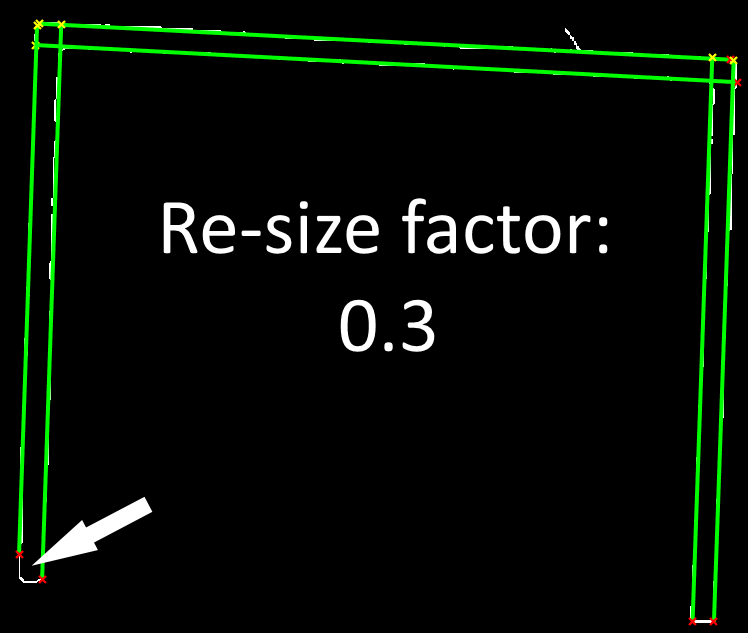
\includegraphics[width=0.73\textwidth]{fig/resize1}
  \caption{Re-size factor: 0.3}
  \label{fig:resize1}
\end{figure}
\begin{figure}[H]
\centering
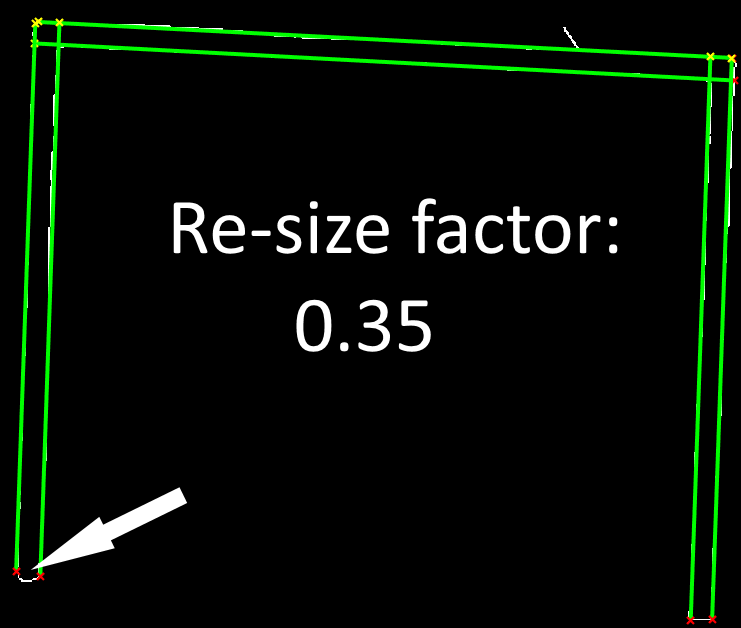
\includegraphics[width=0.73\textwidth]{fig/resize2}
  \caption{Re-size factor: 0.35}
  \label{fig:resize2}
\end{figure}
Figure \ref{fig:resize1} and \ref{fig:resize2} illustrates that a change in the re-sizing factor can lead to a worse Hough transform of wall segments. Looking at the leftmost wall edge, Figure \ref{fig:resize1} has computed a longer wall segment than that of Figure \ref{fig:resize2}. The edge detection algorithm still detects all the wall segments, but the Hough transform outputs two different edge segments depending on the scaling factor. This might lead to an incomplete mapping of the maze.\\

\textbf{Potential solutions}:
\begin{itemize}
\item Capture several pictures of the maze and utilize averaging of the Hough transform
\item Tune the Hough transform for a specific image sensor height
\item Utilize a different method of collecting edge segments; does the system actually need Hough transform?
\item Shorten the edge linking, such that we get more wall segments, but smaller
\end{itemize}

\subsection{Lens distortion}
In Section \ref{lens} I tested the accuracy of our algorithm when moving the maze away from the focal center of the image. The result was that we have an increase of computed wall length as the maze approaches the edge of the image. The likely cause for this is lens distortion, and is a well researched subject in image processing. To correct for this, parameters of the camera needs to be extracted and corrected for in the image.\\

\textbf{Potential solutions}
\begin{itemize}
\item Use the built-in lens Camera Calibrator in Matlab together with images of a checkerboard pattern (Figure \ref{fig:checker}) to extract camera parameters. The checkerboard pattern is taped on an even surface and several images are captured of the pattern and put in the Camera Calibrator to extract the parameter.
\item Use more a more advanced camera calibration method as described in \cite{lens}
\item Use an image sensor with optics that do not distort the image 
\item Define an area away from the focal center and crop it to reduce the distortion along the edges
\end{itemize}
\begin{figure}[H]
\centering
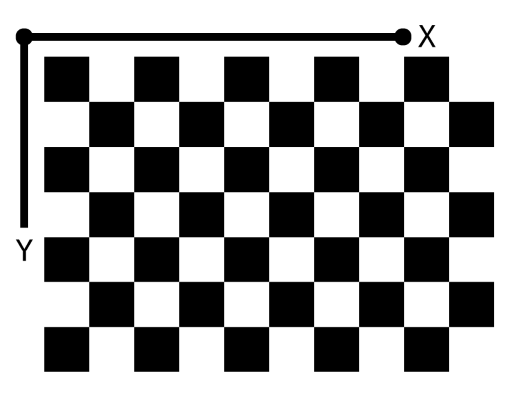
\includegraphics[width=0.73\textwidth]{fig/checker}
  \caption{Checkerboard pattern for lens distortion correction}
  \label{fig:checker}
\end{figure}

\subsection{Bad tuning parameters for different heights}
As described in Section \ref{varyingheight} the Canny edge detection algorithm parameters needed to be tuned for each height. This might lead to bad tuning parameters if the height of the image sensor changes when in the process of capturing images of the maze. Bad tuning parameters means that some of the walls might not be registered by the algorithm, and thus not mapped. The reason this happens is because the intensity value function (Figure \ref{fig:derivatives}) of the edges will become longer the closer the image is taken to the edge. To combat this there are a couple of things one can try:\\

\textbf{Potential solutions}
\begin{itemize}
\item Tune the parameters as a function of image height. This is very difficult and I have not been able to find a good function for this.
\item Assume that the image sensor takes images from the same height in the application
\end{itemize}











